% ============================================================
%  CAPÍTULO 3 – MATERIALES Y MÉTODOS
% -----------------------------------------------------------
\subsection{Arquitectura general del sistema}
\label{subsec:arquitectura_general_del_sistema}
% -----------------------------------------------------------
El sistema se organiza en cinco capas funcionales que cubren el ciclo completo desde la obtención de los datos hasta la presentación de resultados al usuario. Esta separación permite que cada componente sea desarrollado, probado y actualizado de forma independiente.

Como se muestra en la Figura~\ref{fig:arquitectura}, la primera capa se ocupa de la adquisición de datos: mediante procesos de \textit{scraping} automatizado se capturan ofertas de empleo, cursos de formación, programas de máster y sus precios asociados. La segunda capa transforma esos datos brutos en información estructurada y comparable, aplicando procesos de normalización textual, enriquecimiento semántico y mapeo sobre una taxonomía de habilidades común. La tercera capa constituye el núcleo analítico del sistema: a partir del CV del usuario construye su perfil profesional, calcula el \textit{skill gap} respecto al rol objetivo y genera las recomendaciones de formación y empleo. La cuarta capa agrupa la evaluación y validación del modelo. La quinta y última capa es la interfaz con el usuario, implementada como aplicación web, donde se presentan los resultados de forma visual, filtrable y explicable.

\begin{figure}[H]
  \centering
  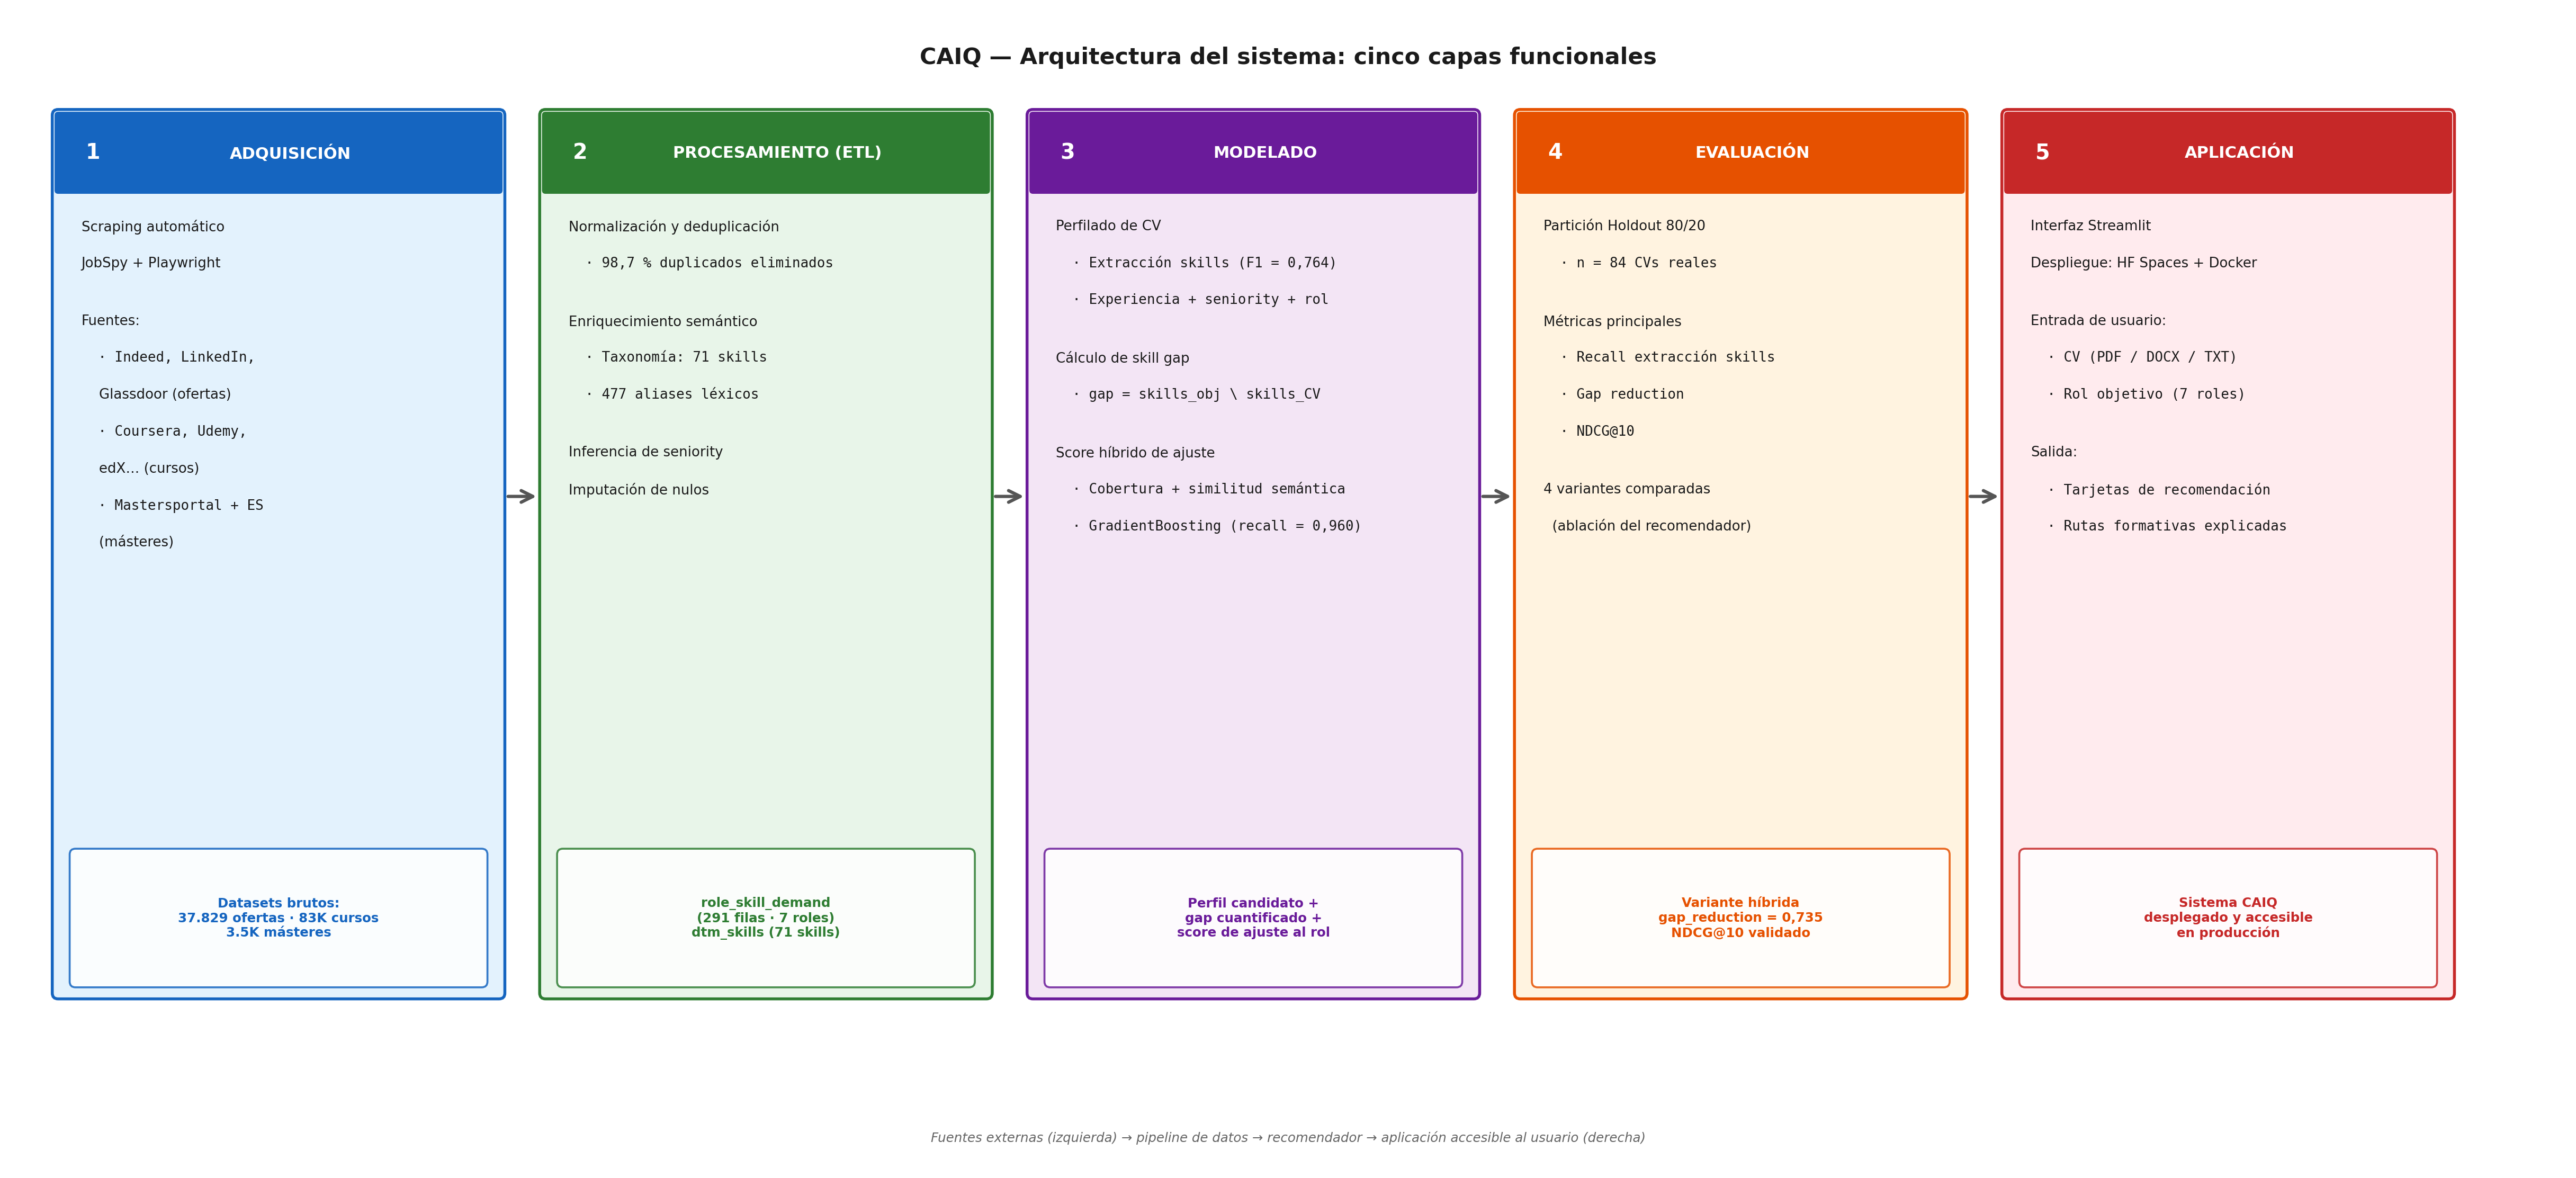
\includegraphics[width=0.95\textwidth]{figures/fig31_arquitectura_caiq}
  \caption{Arquitectura general del sistema CAIQ organizada en cinco capas funcionales: adquisición, procesamiento, modelado, evaluación y aplicación.}
  \label{fig:arquitectura}
\end{figure}

El sistema articula dos flujos de datos que confluyen en el motor de recomendación. Por un lado, los datos externos (ofertas de empleo, cursos y programas de máster) se procesan a través del \textit{pipeline} ETL (\textit{Extract, Transform, Load}) hasta convertirse en \textit{datasets} estructurados y depurados. Por otro, la carga del CV del usuario activa un flujo paralelo que extrae su perfil profesional y estima el \textit{skill gap}. Ambos flujos se integran en la capa de modelado, cuyos resultados se presentan al usuario mediante la interfaz web.

% -----------------------------------------------------------
\subsection{\textit{Stack} tecnológico y decisiones de diseño}
\label{subsec:stack_tecnologico}
% -----------------------------------------------------------
En la Tabla~\ref{tab:stack} se muestra el \textit{stack} tecnológico del sistema y la justificación de cada componente. Los criterios de selección fueron tres: adecuación técnica a la tarea, viabilidad en un entorno sin GPU dedicada, y compatibilidad con el ecosistema Python habitual en proyectos de ciencia de datos.

\begin{table}[H]
  \caption{\textit{Stack} tecnológico del sistema CAIQ y justificación de cada decisión de diseño.}
  \label{tab:stack}
  \centering
  \footnotesize
  \begin{tabular}{|p{3.8cm}|p{4.5cm}|p{6.2cm}|}
    \hline
    \rowcolor{gray!15}
    \textbf{Componente} & \textbf{Tecnología} & \textbf{Justificación} \\
    \hline
    Lenguaje principal    & Python 3.11                          & Ecosistema ML/NLP maduro; tipado moderno \\
    \hline
    \textit{Scraping} de empleo    & \texttt{JobSpy}                               & Unifica \texttt{LinkedIn}, \texttt{Indeed} y \texttt{Glassdoor} en una sola API sin credenciales \\
    \hline
    Extracción de PDF     & \texttt{pypdf} + \texttt{pdfplumber} + \texttt{PyMuPDF}         & Cadena en cascada; robustez ante PDFs complejos o escaneados \\
    \hline
    Renderizado dinámico  & \texttt{Playwright}                           & \textit{Scraping} de páginas con JavaScript y carga diferida \\
    \hline
    \textit{Embeddings} semánticos & \texttt{sentence-transformers}                & Estado del arte en similitud de texto; modelos descargables \\
    \hline
    Modelo de \textit{embeddings}  & \texttt{paraphrase-multilingual-} \newline \texttt{MiniLM-L12-v2} & Soporte nativo español e inglés; 384 dimensiones; equilibrio calidad/velocidad sin GPU \\
    \hline
    Interfaz web          & \texttt{Streamlit} 1.x                        & Prototipado rápido sin capa \textit{frontend} separada \\
    \hline
    Almacenamiento        & CSV + \texttt{Pickle}                         & Sin servidor; máxima portabilidad y reproducibilidad \\
    \hline
    Despliegue            & Hugging Face Spaces + Docker         & Gratuito; entorno reproducible; acceso público sin infraestructura propia \\
    \hline
  \end{tabular}
\end{table}

En la capa de adquisición, \texttt{JobSpy} centraliza el \textit{scraping} de ofertas de empleo y \texttt{Playwright} gestiona la extracción de precios de cursos en plataformas con renderizado dinámico. El procesamiento y análisis se apoya en \texttt{Pandas} y \texttt{NumPy} para la manipulación tabular, y en \texttt{scikit-learn} para las tareas de modelado y evaluación.

La capa de modelado incorpora dos decisiones específicas. Por un lado, la representación semántica se resuelve con el modelo \texttt{paraphrase-multilingual-MiniLM-L12-v2} (Reimers \& Gurevych, 2019) de la librería \texttt{sentence-transformers}: este modelo ofrece \textit{embeddings} de buena calidad con un coste computacional compatible con CPU, lo que lo hace idóneo para un entorno de despliegue sin GPU. Por otro, la extracción de texto de currículums combina \texttt{pypdf}, \texttt{pdfplumber} y \texttt{PyMuPDF} en cascada, de forma que si un método no obtiene resultados limpios el sistema recurre automáticamente al siguiente, mejorando la robustez frente a documentos con estructuras irregulares.

La interfaz se construye sobre \texttt{Streamlit}, que permite desarrollar aplicaciones web interactivas en Python sin necesidad de mantener un \textit{stack frontend} independiente. El despliegue se realiza mediante un contenedor Docker alojado en Hugging Face Spaces, lo que garantiza reproducibilidad y acceso público sin infraestructura propia. El \textit{stack} se organiza de forma coherente con las cinco capas del sistema descritas en el apartado anterior.

% -----------------------------------------------------------
\subsection{Fuentes de datos}
\label{subsec:fuentes_de_datos}
% -----------------------------------------------------------
En este trabajo se utilizan tres fuentes de información complementarias, cada una orientada a cubrir una necesidad distinta dentro del proceso de recomendación: \textbf{Ofertas de empleo}, \textbf{Programas formativos} y \textbf{CV del usuario}.

\textbf{Ofertas de empleo.} Las ofertas publicadas en portales de empleo permiten observar qué perfiles se buscan en el mercado, qué habilidades aparecen con más frecuencia y cómo se formulan los requisitos. Rahhal et al. (2024) señalan en su revisión sistemática que este tipo de datos constituye una de las fuentes más directas para estudiar la demanda real de competencias. La recogida de ofertas se realiza mediante \textit{scraping} en tres plataformas: \texttt{Indeed}, \texttt{LinkedIn} y \texttt{Glassdoor}, seleccionadas por su volumen, la diversidad geográfica y sectorial que ofrecen, y la viabilidad técnica del acceso.

Como se muestra en la Figura~\ref{fig:dist_fuentes_portal}, el \textit{snapshot} operativo está compuesto por 37.829 ofertas de empleo tras el proceso de limpieza y deduplicación, correspondientes al período febrero~2024 -- mayo~2026, con mayor concentración en el período octubre~2025 -- mayo~2026. Las ofertas se distribuyen entre \texttt{Indeed} (25.643; 67,8\,\%), \texttt{LinkedIn} (10.917; 28,9\,\%) y \texttt{Glassdoor} (1.269; 3,4\,\%).

\begin{figure}[H]
  \centering
  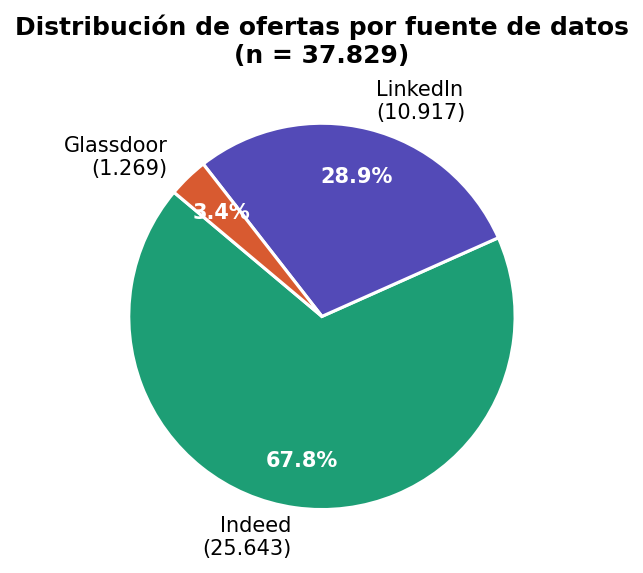
\includegraphics[width=0.65\textwidth]{figures/fig35_dist_fuentes}
  \caption{Distribución de ofertas de empleo por portal de origen tras el proceso de \textit{scraping} y deduplicación.}
  \label{fig:dist_fuentes_portal}
\end{figure}

La Figura~\ref{fig:evolucion_temporal} muestra la evolución mensual del volumen de ofertas recopiladas a lo largo del período de recogida de datos. El proceso se desarrolló en dos fases claramente diferenciadas. La \textbf{fase de recolección intensiva} (octubre~2025 -- febrero~2026) incorporó el grueso del corpus mediante ciclos de \textit{scraping} de alta frecuencia, alcanzando un pico de 18.665 ofertas en febrero~2026. A partir de abril~2026 el proceso entró en la \textbf{fase de mantenimiento incremental}, con una cadencia semanal estabilizada entre 1.750 y 2.155 ofertas mensuales, suficiente para reflejar las variaciones reales del mercado sin reconstruir el \textit{dataset} desde cero. El detalle cuantitativo del proceso (número de ciclos, registros brutos y tasa de recapturas descartadas) se presenta en la Sección~\ref{subsec:resultados_obj2}.

\begin{figure}[H]
  \centering
  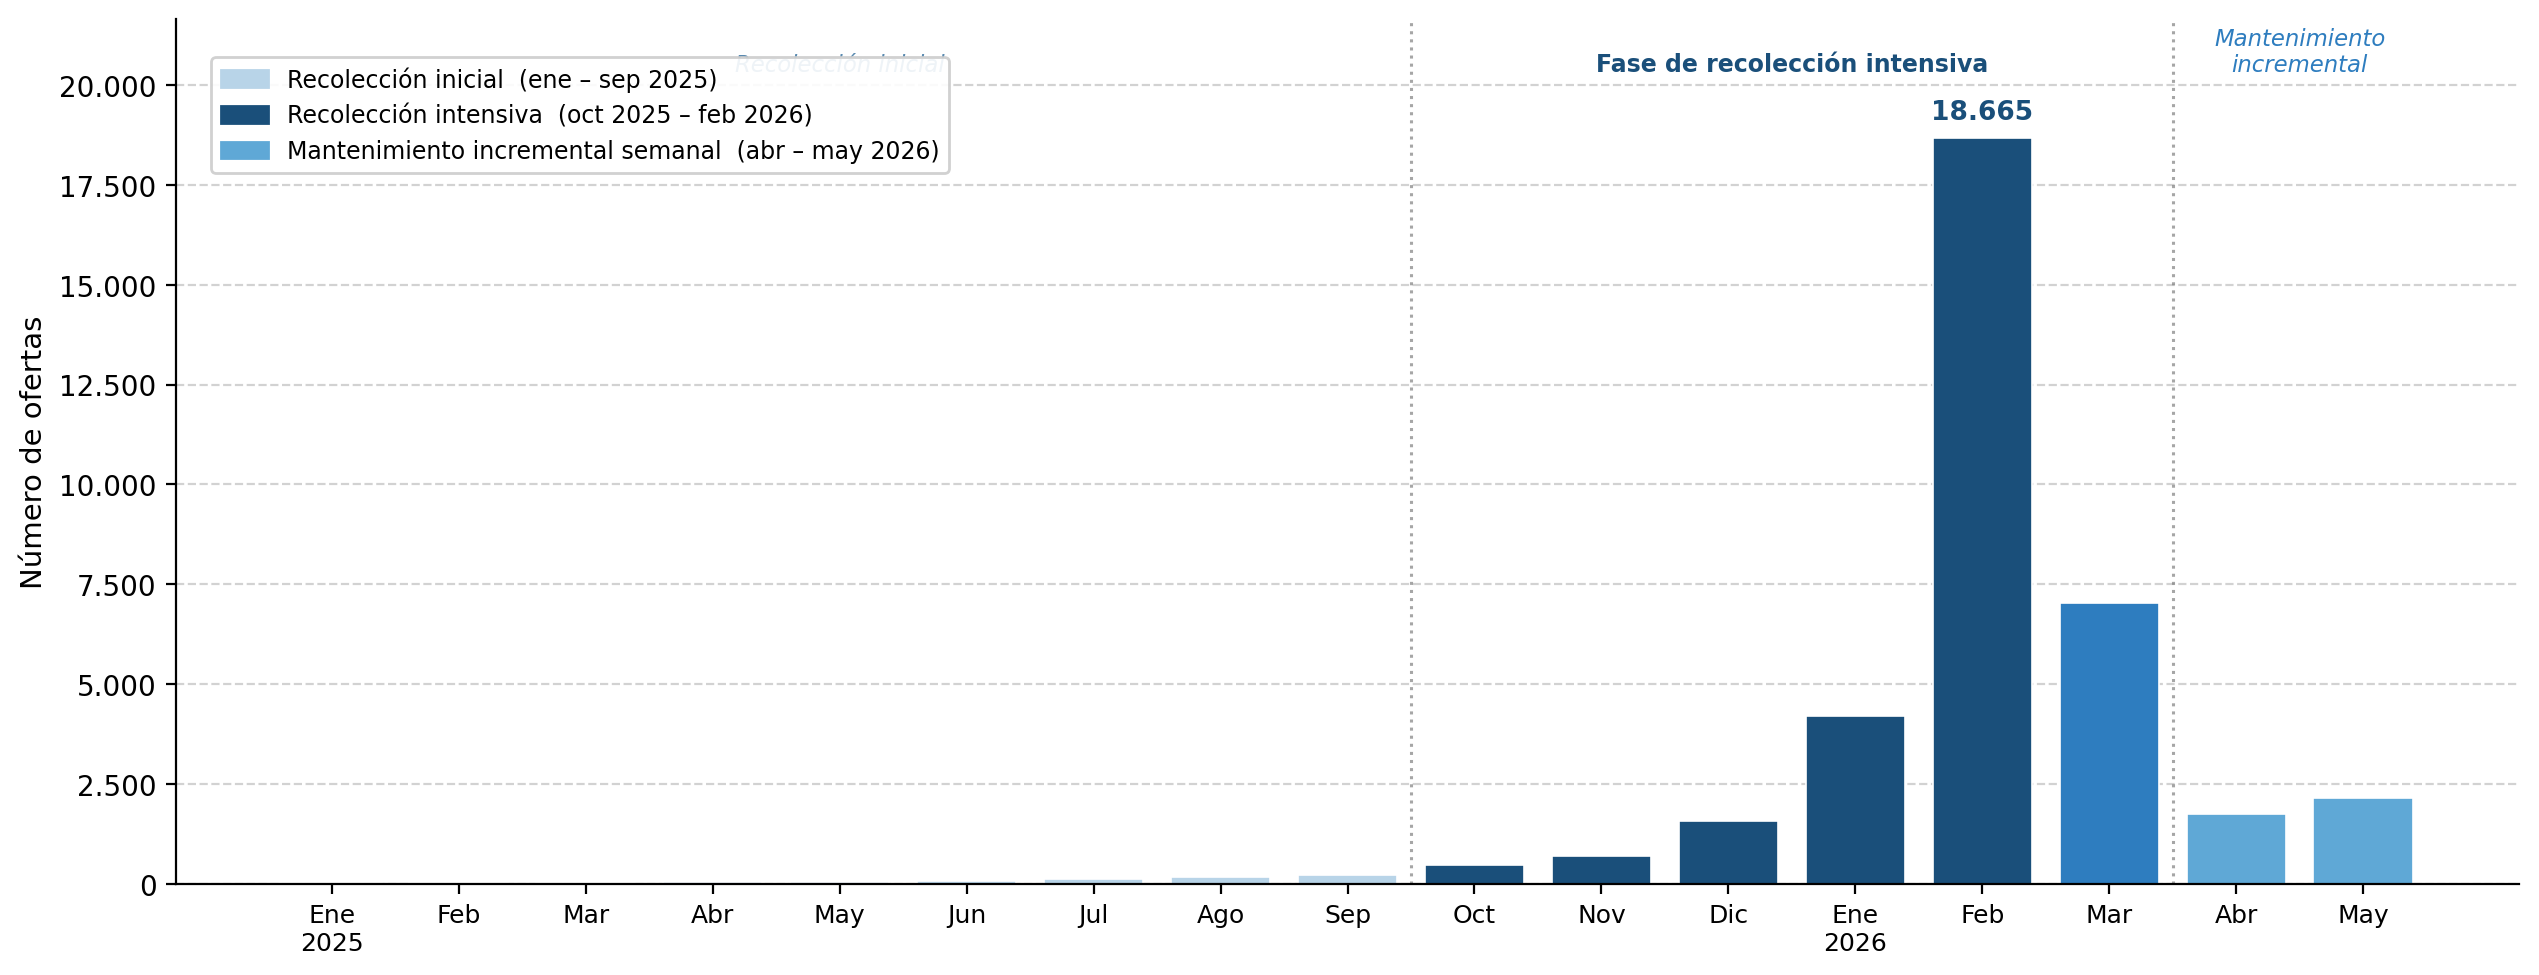
\includegraphics[width=0.95\textwidth]{figures/fig_evolucion_temporal}
  \caption{Evolución mensual del número de ofertas de empleo recopiladas mediante \textit{scraping} (enero~2025 -- mayo~2026). Las barras oscuras corresponden a la fase de recolección intensiva (oct.~2025 -- feb.~2026); las barras claras, a la fase de mantenimiento incremental semanal (abr.~2026 -- may.~2026).}
  \label{fig:evolucion_temporal}
\end{figure}

La Figura~\ref{fig:dist_geografica} muestra la distribución geográfica del corpus. La mayor parte de las ofertas proceden de Estados Unidos (66,8\,\%), reflejo del peso de \texttt{Indeed} y \texttt{LinkedIn} en el mercado anglosajón y de la internacionalización de los perfiles de datos. España representa el 3,6\,\% del corpus (1.369 ofertas), lo que garantiza representatividad del mercado local junto con una perspectiva comparada con otros mercados.

\begin{figure}[H]
  \centering
  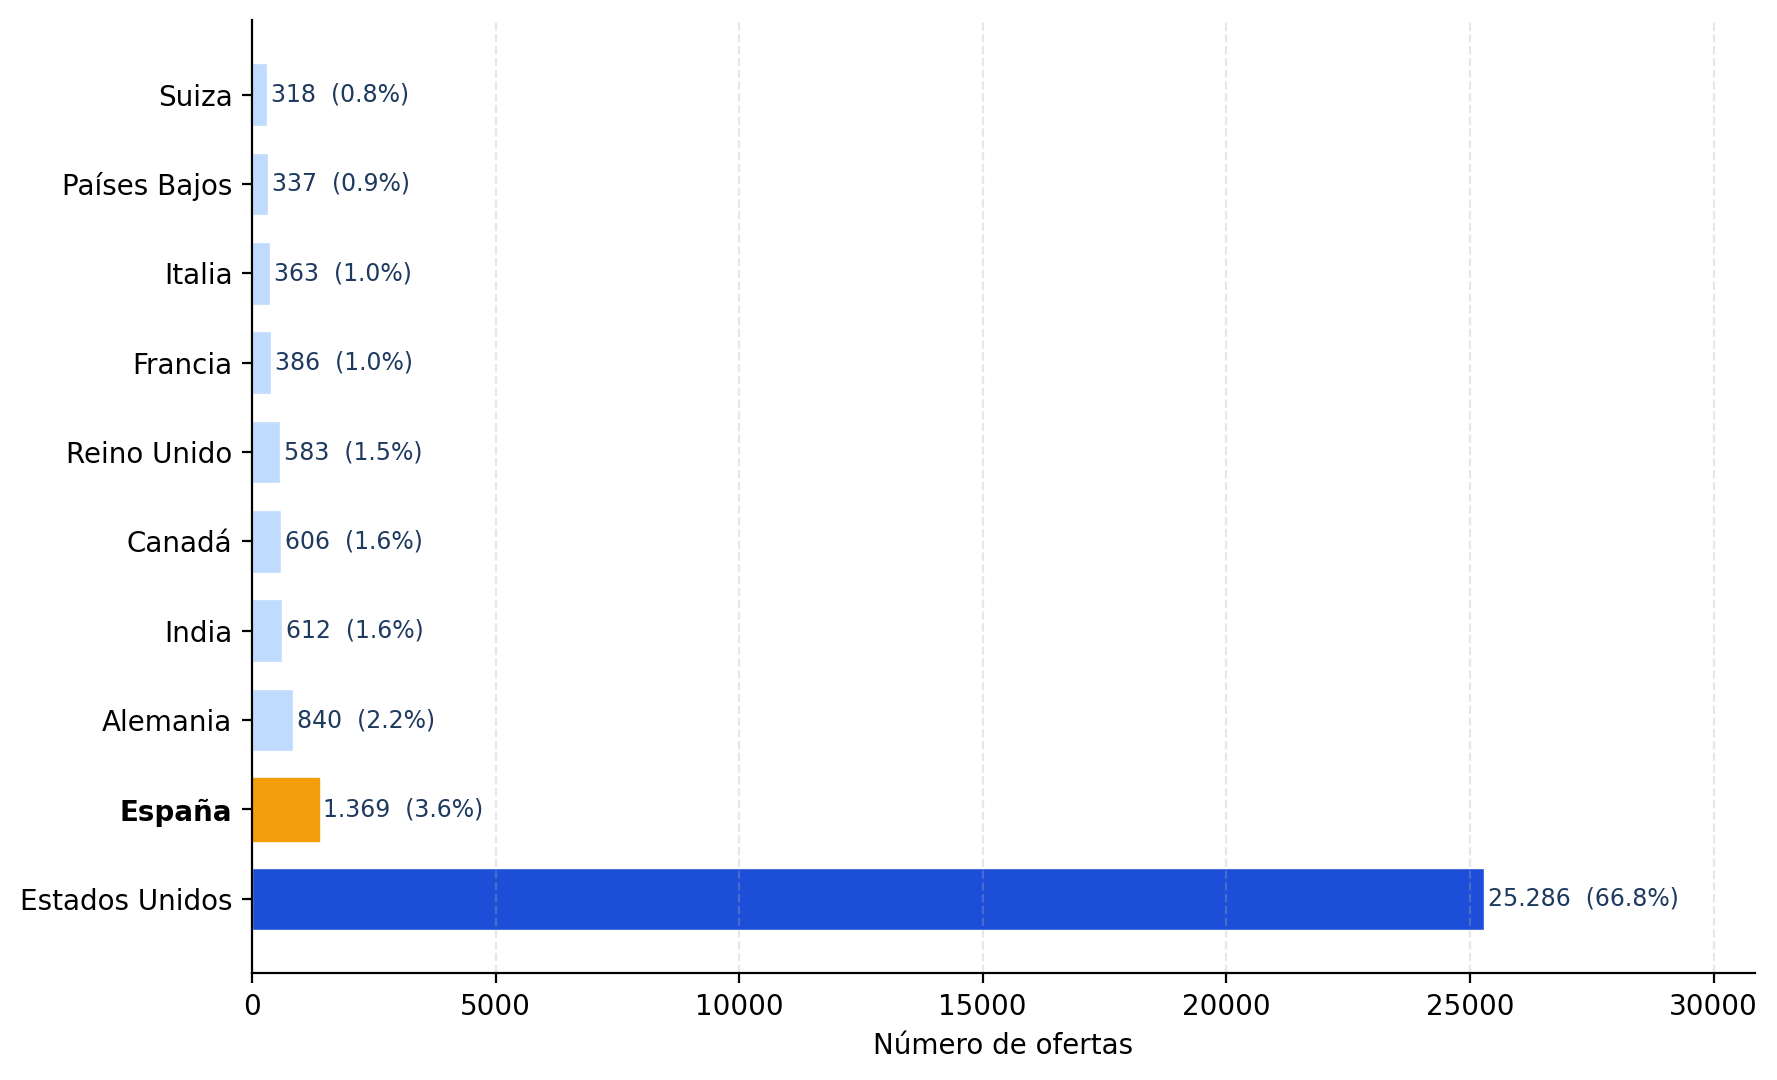
\includegraphics[width=0.82\textwidth]{figures/fig_distribucion_geografica}
  \caption{Distribución de las ofertas de empleo por país de publicación (top 10). España aparece destacada en naranja. Se excluyen registros sin localización identificable (3,5\,\% del corpus).}
  \label{fig:dist_geografica}
\end{figure}

Este corpus se complementa en la capa semántica con una tabla \texttt{role\_skill\_demand} extendida a siete familias analíticas: \texttt{data\_analyst}, \texttt{data\_engineer}, \texttt{data\_scientist}, \texttt{ml\_engineer}, \texttt{business\_intelligence}, \texttt{mlops} y \texttt{other\_data\_role}. Como se muestra en la Figura~\ref{fig:dist_roles}, la distribución por familia de rol refleja la mayor representación de perfiles de análisis e ingeniería de datos.

\begin{figure}[H]
  \centering
  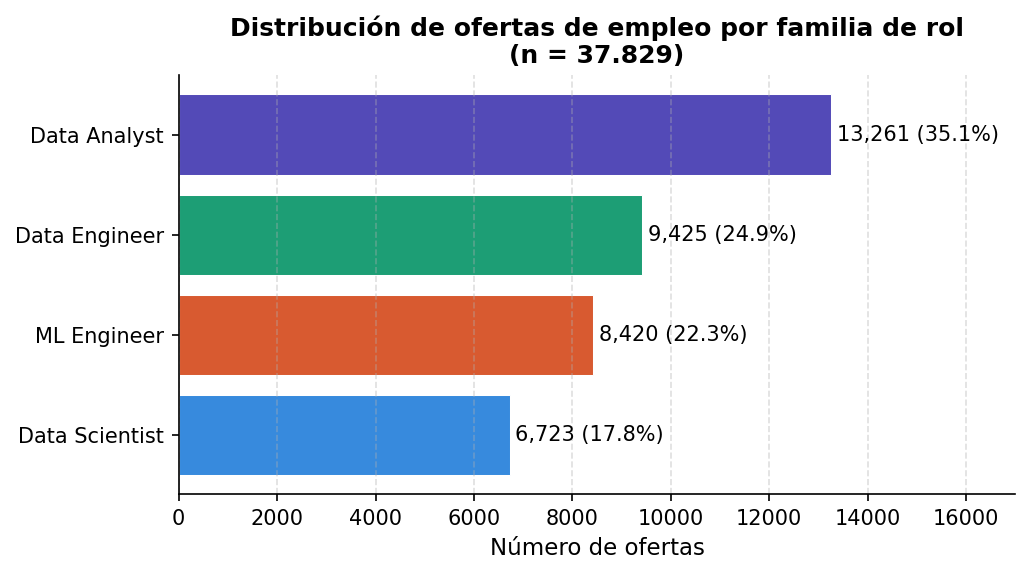
\includegraphics[width=0.80\textwidth]{figures/fig32_dist_role_family}
  \caption{Distribución de ofertas de empleo por familia de rol en el \textit{dataset} consolidado.}
  \label{fig:dist_roles}
\end{figure}

\textbf{Programas formativos.} La oferta formativa se divide en dos grupos: cursos \textit{online} y másteres. El catálogo de cursos integra 89.332 registros procedentes de \texttt{Udemy}, enriquecidos en una segunda fase con cursos de \texttt{Coursera}, \texttt{edX}, \texttt{Udacity}, \texttt{Skillshare} y \texttt{Simplilearn}. La valoración media de los cursos es de 4,39 sobre 5 (desviación estándar 0,32), distribución que no discrimina suficientemente entre cursos. Por eso, el sistema otorga mayor peso a la cobertura de \textit{skills} y a la similitud semántica que a la popularidad (Burke, 2002).

El catálogo de másteres contiene 3.503 programas de posgrado procedentes de \texttt{Mastersportal.eu} y universidades e instituciones españolas. Tras la incorporación de 78 programas de universidades y escuelas de negocio españolas, el catálogo cuenta con 96 másteres ubicados en España (el 2,7\,\% del total), con una duración media de 16 meses.

\textbf{CV del usuario.} El currículum del usuario no se captura ni almacena de forma centralizada, sino que se procesa en tiempo de ejecución. Esta decisión responde a criterios de privacidad: el CV constituye el punto de partida personalizado a partir del cual se genera el análisis. Su tratamiento detallado se desarrolla en la Sección~\ref{subsec:modelado_cv}.

% -----------------------------------------------------------
\subsection{\textit{Pipeline} de \textit{scraping} y actualización incremental}
\label{subsec:pipeline_scraping}
% -----------------------------------------------------------
La recogida de ofertas se ejecuta como un proceso incremental que incorpora nuevas observaciones periódicamente, sin reconstruir el \textit{dataset} desde cero en cada ciclo. Las fuentes consultadas son \texttt{Indeed}, \texttt{LinkedIn} y \texttt{Glassdoor}; sobre cada una se lanzan consultas independientes con los términos de búsqueda correspondientes a las familias de rol del sistema (\textit{data scientist}, \textit{data analyst}, \textit{data engineer}, \textit{machine learning engineer}, \textit{business intelligence analyst}, entre otros). La ejecución de consultas por separado hace que, si una fuente falla o devuelve resultados vacíos, el resto del ciclo continúe sin interrupciones.

Cada ejecución genera un archivo intermedio con las ofertas recuperadas, que se compara con el \textit{dataset} maestro para incorporar únicamente las novedades. La deduplicación se basa en la URL de la oferta cuando está disponible, y en una clave compuesta por portal, título, empresa y localización cuando no lo está.

\textbf{Umbral de antigüedad.} La antigüedad máxima admisible para incorporar una oferta se fija en 30 días. Burning Glass Technologies et al. (2017) estiman que la vida media de una oferta técnica activa es inferior a cuatro semanas, de modo que retener ofertas más antiguas aumentaría el ruido sin añadir señal actualizada sobre el estado real del mercado.

\textbf{Determinación de la cadencia de actualización.} La periodicidad del \textit{scraping} se fija en una ejecución semanal, resultado de ponderar tres criterios contrapuestos. En primer lugar, el criterio de cobertura: con una vida media de oferta activa inferior a cuatro semanas (Burning Glass Technologies et al., 2017), una cadencia semanal permite capturar cada posición antes de que expire en al menos el 75\,\% de los casos, mientras que una cadencia quincenal o mensual perdería sistemáticamente las ofertas con menor tiempo de exposición (aquellas cubiertas en 1--2 semanas, frecuentes en perfiles técnicos con alta demanda). En segundo lugar, el criterio de viabilidad técnica: los tres portales consultados (\texttt{Indeed}, \texttt{LinkedIn}, \texttt{Glassdoor}) aplican limitaciones de tasa implícitas a través de la capa de abstracción de \texttt{JobSpy}; una cadencia diaria requeriría rotación de proxies y una infraestructura de evasión de detección que excede el alcance del presente trabajo. En tercer lugar, el criterio de estabilidad de señal: el mercado laboral de datos no experimenta variaciones diarias estadísticamente significativas en la distribución de competencias demandadas; la semana es la unidad mínima con suficiente varianza interperiódica para que el \textit{delta} de nuevas ofertas sea informativo (Carnevale et al., 2015). La combinación de estos tres criterios posiciona la cadencia semanal como el equilibrio adecuado entre actualización real del \textit{snapshot}, cobertura del espacio de ofertas activas y viabilidad operativa sin infraestructura dedicada.

Durante el período de construcción del sistema (11 de marzo -- 22 de mayo de 2026, 71 días) se ejecutaron de forma recurrente ciclos de \textit{scraping} siguiendo este procedimiento incremental. Los resultados operativos del proceso —número de ciclos realizados, volumen medio de ofertas por ciclo y cobertura temporal del \textit{snapshot} final— se presentan en la Sección~\ref{subsec:resultados_obj2}.

\textbf{Mantenimiento y depuración del corpus.} Para garantizar que el corpus refleja la oferta activa en el mercado y no acumula entradas obsoletas, el \textit{pipeline} aplica dos mecanismos complementarios de depuración en cada ejecución semanal. El primero es la \textbf{caducidad temporal}: durante la fusión con el histórico, se descartan automáticamente todas las ofertas con \texttt{date\_posted} superior a 90 días respecto a la fecha de ejecución (\texttt{keep\_days\,=\,90}), eliminando entradas que, con alta probabilidad, ya no están disponibles en los portales de origen. El segundo es la \textbf{verificación activa de URLs}: mediante peticiones HTTP de tipo HEAD a la URL de cada oferta, el sistema comprueba si el enlace sigue siendo válido. En el caso de \texttt{LinkedIn}, se verifica además que la URL final de redirección continúa apuntando a la ruta \texttt{/jobs/view/}, ya que las ofertas eliminadas son redirigidas fuera de esa ruta. El resultado de cada verificación se almacena en un archivo de caché persistente (\texttt{job\_url\_status.csv}) con las categorías \textit{active}, \textit{dead}, \textit{blocked} o \textit{unknown}, y con un tiempo de vida de siete días (\texttt{ttl\,=\,7\,d}) para evitar comprobaciones innecesarias de URLs recientes. Por razones de eficiencia, el número máximo de URLs verificadas por ciclo se limita a 300, dando prioridad a las publicadas en los últimos 60 días y a aquellas cuyo estado no ha sido comprobado recientemente. Las ofertas marcadas como \textit{dead} quedan excluidas de las recomendaciones en la capa de aplicación.

% -----------------------------------------------------------
\subsection{Proceso ETL: limpieza, normalización y enriquecimiento}
\label{subsec:proceso_etl}
% -----------------------------------------------------------
El proceso ETL (\textit{Extract, Transform, Load}) transforma los registros brutos procedentes de las distintas fuentes en \textit{datasets} estructurados, homogéneos y enriquecidos con variables derivadas. La Tabla~\ref{tab:tabla3_1} ilustra el estado del \textit{dataset} de ofertas antes del proceso, con títulos heterogéneos, localizaciones no normalizadas y campos de nivel ausentes.

\begin{table}[H]
  \caption{\textit{Dataset} de ofertas antes de la fase ETL. Registros ilustrativos del estado bruto.}
  \label{tab:tabla3_1}
  \centering
  \footnotesize
  \begin{tabular}{|p{3.2cm}|p{2.8cm}|p{2.0cm}|p{5.5cm}|}
    \hline
    \rowcolor{gray!15}
    \textbf{title} & \textbf{company} & \textbf{location} & \textbf{description (extracto)} \\
    \hline
    Data Scientist & Acme Corp & New York, NY & We are looking for a passionate DS\ldots \\
    Sr. Data Scientist & --- & Remote (US) & Join our team! Must have Python, SQL\ldots \\
    Data Scientist / Analyst & GlobalTech & London, UK & Exciting opportunity for a data\ldots \\
    Machine Learning Eng. & StartupXYZ & San Francisco & ML Engineer needed for NLP projects\ldots \\
    \hline
  \end{tabular}
\end{table}

El proceso se estructura en tres capas progresivas.

\begin{itemize}
  \item \textbf{Limpieza y normalización.} La primera capa consolida la información procedente de todas las fuentes bajo un esquema común. Se aplica una rutina de normalización textual para limpiar espacios sobrantes, unificar cadenas, tratar valores nulos y estabilizar el formato de todos los campos de texto. Los registros con campos obligatorios ausentes se descartan. La deduplicación emplea la URL de la oferta como clave primaria; en su ausencia, se utiliza la combinación de portal, título, empresa y localización.
  \item \textbf{Estructuración semántica.} A partir de la base curada se construye una representación textual unificada para cada entidad. Esta representación es la entrada directa a la extracción de competencias y al cálculo de similitudes semánticas.
  \item \textbf{Enriquecimiento y variables derivadas.} Esta capa añade las variables analíticas que habilitan el motor de recomendación. La clasificación por familia de rol (\texttt{role\_family}) se infiere principalmente del título del puesto. La extracción de \textit{skills} se realiza mediante la taxonomía controlada descrita en la Sección~\ref{subsubsec:extraccion_competencias}, generando las tablas \texttt{candidate\_skills}, \texttt{job\_skills}, \texttt{master\_skills} y \texttt{course\_skills}. Las variables de modalidad de trabajo (\texttt{work\_mode}), tipo de empleo (\texttt{employment\_type}) y nivel de \textit{seniority} se derivan mediante reglas heurísticas sobre el texto. Las duraciones se normalizan a meses y el precio de matrícula de másteres se convierte a euros/año.
\end{itemize}

La Tabla~\ref{tab:tabla3_2} muestra el \textit{dataset} resultante tras el ETL. El impacto cuantitativo del proceso se presenta en la Sección~\ref{subsec:resultados_obj2}.

\begin{table}[H]
  \caption{\textit{Dataset} de ofertas después de la fase ETL. Registros ilustrativos con variables normalizadas y enriquecidas.}
  \label{tab:tabla3_2}
  \centering
  \footnotesize
  \begin{tabular}{|p{3.0cm}|p{2.2cm}|p{1.8cm}|p{2.0cm}|p{4.5cm}|}
    \hline
    \rowcolor{gray!15}
    \textbf{title\_norm} & \textbf{role\_family} & \textbf{seniority} & \textbf{work\_mode} & \textbf{\textit{skills} (extracto)} \\
    \hline
    Data Scientist       & \texttt{data\_scientist} & mid    & remote  & python, sql, machine learning \\
    Senior Data Scientist & \texttt{data\_scientist} & senior & remote  & python, deep learning, pytorch \\
    Data Analyst         & \texttt{data\_analyst}   & mid    & hybrid  & sql, tableau, excel \\
    ML Engineer          & \texttt{ml\_engineer}    & mid    & on-site & python, mlops, docker, kubernetes \\
    \hline
  \end{tabular}
\end{table}

Los valores ausentes que persisten tras el ETL se conservan sin imputación: los portales no exponen estos campos en sus páginas públicas de forma sistemática, de modo que su ausencia es una limitación inherente a la fuente original, no corregible mediante técnicas de imputación sin introducir sesgos.

% -----------------------------------------------------------
\subsection{Modelado del perfil profesional}
\label{subsec:modelado_cv}
% -----------------------------------------------------------
\subsubsection{Ingesta y preprocesamiento de documentos curriculares}
\label{subsubsec:ingesta_cv}
El módulo de ingesta acepta documentos en PDF, DOCX y TXT, aplicando una estrategia de lectura específica según el tipo de archivo.

\begin{itemize}
  \item \textbf{\textit{Parsing} por formato.} Los documentos de texto plano se leen directamente. Los DOCX se procesan reconstruyendo el contenido a partir de la estructura XML del documento. Los PDF se procesan mediante una cadena de librerías (\texttt{pypdf}, \texttt{pdfplumber}, \texttt{PyMuPDF}) con mecanismos de respaldo sucesivos para maximizar la extracción limpia ante documentos con estructuras irregulares.
  \item \textbf{Normalización textual.} Sobre el texto extraído se aplican: corrección de caracteres espaciados frecuentes en PDFs exportados, unificación de espacios y saltos de línea, y eliminación de fragmentos vacíos o redundantes.
  \item \textbf{Segmentación semántica.} El texto normalizado se organiza en bloques semánticos (experiencia, formación, habilidades, proyectos, certificaciones) utilizando encabezados y patrones léxicos como señales de estructura. Esta segmentación permite asociar cada competencia detectada a su fuente dentro del CV.
\end{itemize}

\subsubsection{Extracción de competencias mediante taxonomía controlada}
\label{subsubsec:extraccion_competencias}
La transformación del texto libre en competencias normalizadas se realiza mediante una taxonomía controlada con reglas de coincidencia léxica. Se descarta el uso de modelos de reconocimiento de entidades (NER) por la ausencia de un corpus de currículos anotados. La taxonomía controlada ofrece ventajas en términos de interpretabilidad, trazabilidad y capacidad de actualización incremental, en línea con los hallazgos de Zhang et al. (2022), que demuestran que modelos apoyados en un vocabulario bien estructurado pueden superar a sistemas más complejos sin esa base.

La taxonomía define un término canónico por competencia acompañado de sus variantes léxicas. Diferentes denominaciones de una misma herramienta (como PowerBI, Power BI o Microsoft Power BI) quedan unificadas bajo \texttt{power\_bi}. Previamente a la extracción, el texto se normaliza (minúsculas, eliminación de acentos) y se identifican coincidencias mediante reglas que minimizan errores por solapamientos léxicos.

La taxonomía se amplió iterativamente de 59 a 71 competencias y de 190 a 477 \textit{aliases} (media de 6,7 por competencia frente a 3,2 inicial). Las incorporaciones más relevantes fueron: \texttt{Kafka}, \texttt{Terraform}, \texttt{MLflow}, \texttt{Linux}/\texttt{bash} y \texttt{FastAPI}. Paralelamente, se enriquecieron los \textit{aliases} en español para mejorar la cobertura en CVs redactados en castellano.

\subsubsection{Inferencia de experiencia, \textit{seniority} y orientación profesional}
\label{subsubsec:inferencia_seniority}
Además de las competencias detectadas, el perfil profesional requiere variables que caractericen la trayectoria del candidato: experiencia acumulada, distribución por dominio técnico, nivel de \textit{seniority} y alineación con las familias de rol del mercado.

\textbf{Estimación de experiencia profesional.} El sistema identifica rangos temporales en el texto mediante expresiones regulares. Todos los rangos se transforman a un índice mensual continuo:
\[
  \texttt{month\_index} = 12 \cdot \texttt{year} + \texttt{month}
\]
La duración total de experiencia se calcula como:
\[
  \texttt{total\_months} = \sum \max(0,\; \texttt{end\_month} - \texttt{start\_month} + 1)
\]
Los intervalos solapados se fusionan antes de agregar para evitar doble conteo. Los rangos se clasifican en experiencia profesional o de prácticas según el contexto léxico próximo. Como resultado se generan: \texttt{experience\_years\_total}, \texttt{experience\_years\_non\_intern} e \texttt{internship\_months\_estimated}.

\textbf{Experiencia relevante por dominio técnico.} La experiencia se distribuye entre siete dominios funcionales: \texttt{data\_analytics}, \texttt{machine\_learning}, \texttt{nlp}, \texttt{llm\_genai}, \texttt{data\_engineering}, \texttt{bi\_reporting} y \texttt{cloud\_mlops\_devops}. La puntuación bruta pondera tres fuentes de señal según su solidez evidencial, siguiendo el principio de que las menciones en la sección de experiencia son más informativas que las de proyectos, y estas más que las de habilidades simplemente declaradas (Alsaif et al., 2022):
\[
  \texttt{raw\_score} = 2{,}0 \cdot \texttt{exp\_hits} + 1{,}2 \cdot \texttt{project\_hits} + 0{,}8 \cdot \texttt{skill\_hits}
\]
La proyección relativa sobre los años totales se calcula como:
\[
  \texttt{domain\_years} = \texttt{exp\_total} \cdot \frac{\texttt{raw}}{\max(\texttt{raw})} \cdot \left(0{,}7 + 0{,}3 \cdot \min\!\left(1,\, \frac{\texttt{raw}}{6}\right)\right)
\]
El factor de saturación introduce una corrección proporcional para dominios con señal débil. Esta forma funcional es una heurística de diseño propia cuya calibración no ha sido validada empíricamente; queda identificada como una línea de trabajo futuro.

\textbf{Inferencia de \textit{seniority}.} El nivel de \textit{seniority} se clasifica mediante señales léxicas explícitas del CV (con prioridad) y umbrales sobre años de experiencia (como \textit{fallback}). La Tabla~\ref{tab:tabla3_3} recoge el conjunto completo de reglas.

\begin{table}[H]
  \caption{Reglas de inferencia de \textit{seniority}. Las señales léxicas tienen prioridad sobre los umbrales numéricos.}
  \label{tab:tabla3_3}
  \centering
  \footnotesize
  \begin{tabular}{|p{2.2cm}|p{5.5cm}|p{3.5cm}|p{2.0cm}|}
    \hline
    \rowcolor{gray!15}
    \textbf{Nivel} & \textbf{Señales léxicas explícitas} & \textbf{Umbral (años exp.)} & \textbf{Confianza} \\
    \hline
    \texttt{lead}   & head, director, lead, principal, vp, chief & $\geq 8$ años              & Alta \\
    \hline
    \texttt{senior} & senior, sr., staff, experienced, experto   & $\geq 6$ años              & Alta \\
    \hline
    \texttt{mid}    & (ninguna señal explícita)                  & $3$--$5$ años              & Media \\
    \hline
    \texttt{junior} & junior, jr., entry level, graduate, trainee & $\leq 2$ años             & Alta \\
    \hline
    \texttt{intern} & intern, internship, prácticas, becario     & (no aplicable)             & Alta \\
    \hline
    \textit{default} & Sin señal léxica y sin años detectados   & ---                        & Baja \\
    \hline
  \end{tabular}
\end{table}

\textbf{Orientación por familia de rol.} El sistema calcula el ajuste del perfil respecto a siete familias de rol: \texttt{data\_analyst}, \texttt{data\_scientist}, \texttt{data\_engineer}, \texttt{ml\_engineer}, \texttt{business\_intelligence}, \texttt{mlops} y \texttt{other\_data\_role}. Las competencias de referencia de cada rol se estructuran en tres bandas de prioridad (\textit{core}, \textit{important} y \textit{complementary}) en función de su \texttt{demand\_ratio}; su definición formal y umbrales se recogen en la Sección~\ref{subsubsec:perfil_objetivo}.

La puntuación de ajuste para cada rol se calcula como:
\[
  \texttt{score} = \frac{0{,}50 \cdot p + 0{,}25 \cdot c_{\text{core}} + 0{,}10 \cdot c_{\text{imp}} + 0{,}05 \cdot c_{\text{comp}}}{0{,}90} \cdot \texttt{penalty\_core}
\]
donde $p$ es la presencia general de \textit{skills} del rol y $c_{\text{core}}$, $c_{\text{imp}}$ y $c_{\text{comp}}$ son las coberturas por banda. Los pesos de esta fórmula reflejan la premisa, documentada en la literatura de recomendación basada en contenido (Burke, 2002), de que las señales de cobertura directa son más informativas que las competencias periféricas. Su calibración empírica queda como línea de trabajo futuro.

\subsubsection{Representación estructurada y vectorial del perfil}
\label{subsubsec:representacion_perfil}
Al término del módulo anterior, el CV queda representado en un objeto \texttt{candidate\_profile} con dos capas. La capa simbólica contiene los campos discretos recogidos en la Tabla~\ref{tab:tabla3_4}: \textit{skills} detectadas, experiencia por dominio, \textit{seniority} y puntuaciones de ajuste por rol. La capa semántica proyecta las \textit{skills} como texto y las codifica mediante \texttt{paraphrase-multilingual-MiniLM-L12-v2} (Reimers \& Gurevych, 2019), generando un vector denso de 384 dimensiones que captura afinidades semánticas que el \textit{matching} léxico estricto no detectaría (Burke, 2002).

\begin{table}[H]
  \caption{Variables de salida del módulo de inferencia del perfil profesional.}
  \label{tab:tabla3_4}
  \centering
  \footnotesize
  \begin{tabular}{|p{4.5cm}|p{2.0cm}|p{7.0cm}|}
    \hline
    \rowcolor{gray!15}
    \textbf{Variable} & \textbf{Tipo} & \textbf{Descripción} \\
    \hline
    \texttt{skills\_detected}              & Lista   & Competencias canónicas detectadas en el CV \\
    \hline
    \texttt{experience\_years\_total}      & Float   & Años de experiencia profesional total estimados \\
    \hline
    \texttt{experience\_years\_relevant}   & Float   & Años de experiencia en roles de datos \\
    \hline
    \texttt{experience\_years\_by\_domain} & Dict    & Distribución de experiencia por dominio técnico \\
    \hline
    \texttt{seniority}                     & Texto   & Nivel inferido: \texttt{intern} / \texttt{junior} / \texttt{mid} / \texttt{senior} / \texttt{lead} \\
    \hline
    \texttt{seniority\_confidence}         & Texto   & Confianza de la inferencia: \texttt{high} / \texttt{medium} / \texttt{low} \\
    \hline
    \texttt{role\_fit\_scores}             & Dict    & Puntuación de ajuste a cada familia de rol (0--1) \\
    \hline
    \texttt{detected\_best\_role}          & Texto   & Familia de rol con mayor ajuste \\
    \hline
    \texttt{embedding}                     & Vector  & Representación semántica densa (384 dims, MiniLM) \\
    \hline
  \end{tabular}
\end{table}

\begin{table}[H]
  \caption{Principales campos del objeto \texttt{candidate\_profile} y su función en el sistema.}
  \label{tab:tabla3_5}
  \centering
  \footnotesize
  \begin{tabular}{|p{4.5cm}|p{2.0cm}|p{7.0cm}|}
    \hline
    \rowcolor{gray!15}
    \textbf{Campo} & \textbf{Capa} & \textbf{Función en el sistema} \\
    \hline
    \texttt{skills\_detected}              & Simbólica & Vector \textit{multi-hot} sobre taxonomía; entrada al cálculo del \textit{gap} \\
    \hline
    \texttt{experience\_years\_total}      & Simbólica & Señal de \textit{seniority} para el motor de recomendación \\
    \hline
    \texttt{experience\_years\_by\_domain} & Simbólica & Filtro de relevancia por dominio técnico \\
    \hline
    \texttt{seniority}                     & Simbólica & Etiqueta de nivel; condiciona el tipo de recomendación \\
    \hline
    \texttt{role\_fit\_scores}             & Simbólica & Puntuación de ajuste multi-rol \\
    \hline
    \texttt{detected\_best\_role}          & Simbólica & Rol con mayor afinidad; usado como rol objetivo por defecto \\
    \hline
    \texttt{embedding}                     & Semántica & Vector denso MiniLM; base del componente semántico del \textit{score} \\
    \hline
    \texttt{raw\_text\_blocks}             & Meta      & Bloques segmentados del CV; usados para trazabilidad \\
    \hline
  \end{tabular}
\end{table}

El perfil se persiste en \texttt{st.session\_state} durante la sesión y se serializa al terminar el flujo en \texttt{recommendation\_summary.json}.

% -----------------------------------------------------------
\subsection{Cálculo del \textit{skill gap} y ajuste al rol objetivo}
\label{subsec:calculo_gap}
% -----------------------------------------------------------
Una vez construido el \texttt{candidate\_profile}, el sistema calcula el \textit{skill gap}: el conjunto ordenado de competencias que el candidato no cubre respecto al perfil objetivo de una familia de rol.

\subsubsection{Construcción del perfil objetivo y priorización de competencias}
\label{subsubsec:perfil_objetivo}
El perfil objetivo de cada rol se construye a partir de la tabla \texttt{role\_skill\_demand}, generada en la capa de enriquecimiento del ETL. Esta tabla recoge las \textit{skills} detectadas en las ofertas de empleo de cada familia y su nivel de demanda agregada. La tabla se amplió de cinco familias iniciales a siete con la incorporación de \texttt{business\_intelligence} y \texttt{mlops}, pasando de 219 a 291 filas.

Para cada rol se utilizan como máximo 40 \textit{skills} objetivo, ordenadas por \texttt{demand\_ratio}:
\[
  \texttt{demand\_ratio} = \frac{\texttt{demand\_count}}{\texttt{role\_job\_count}}
\]

Las competencias se clasifican en tres bandas, recogidas en la Tabla~\ref{tab:tabla3_7}:
\begin{itemize}
  \item \textbf{Banda \textit{core}}: competencias presentes en más del 35\,\% de las ofertas del rol (\texttt{demand\_ratio} $\geq 0{,}35$, o las tres primeras si ninguna alcanza ese umbral).
  \item \textbf{Banda \textit{important}}: competencias con $0{,}15 \leq$ \texttt{demand\_ratio} $< 0{,}35$.
  \item \textbf{Banda \textit{complementary}}: competencias diferenciales o emergentes (\texttt{demand\_ratio} $< 0{,}15$).
\end{itemize}

\begin{table}[H]
  \caption{Clasificación de competencias objetivo por banda y peso asociado en el cálculo del \textit{skill gap}.}
  \label{tab:tabla3_7}
  \centering
  \footnotesize
  \begin{tabular}{|p{2.5cm}|p{4.5cm}|p{2.0cm}|p{4.5cm}|}
    \hline
    \rowcolor{gray!15}
    \textbf{Banda} & \textbf{Criterio (\texttt{demand\_ratio})} & \textbf{Peso} & \textbf{Interpretación} \\
    \hline
    \textit{core}          & $\geq 0{,}35$ (o top-3 del rol)  & 2{,}0 & Competencia estructural del rol \\
    \hline
    \textit{important}     & $0{,}15$--$0{,}34$               & 1{,}0 & Competencia relevante no estructural \\
    \hline
    \textit{complementary} & $< 0{,}15$                       & 0{,}5 & Competencia diferencial o emergente \\
    \hline
  \end{tabular}
\end{table}

\subsubsection{Cálculo del \textit{gap}, cobertura y puntuación de ajuste}
\label{subsubsec:calculo_gap_detalle}
El \textit{gap} inicial se calcula como la diferencia de conjuntos entre las competencias del rol objetivo y las del candidato:
\[
  \texttt{gap} = \texttt{skills\_objetivo} \setminus \texttt{skills\_candidato}
\]
El resultado se ordena por \texttt{demand\_ratio}, priorizando las carencias de mayor impacto. Para cada banda se calcula la cobertura ponderada:
\[
  \texttt{coverage\_banda} = \frac{\sum \texttt{peso} \cdot \mathbb{1}[\text{\textit{skill} presente}]}{\sum \texttt{peso} \cdot \mathbb{1}[\text{\textit{skill} en banda}]}
\]

La Tabla~\ref{tab:tabla3_8} recoge los campos de salida de esta fase.

\begin{table}[H]
  \caption{Campos principales de salida del módulo de cálculo del \textit{skill gap}.}
  \label{tab:tabla3_8}
  \centering
  \footnotesize
  \begin{tabular}{|p{4.5cm}|p{2.0cm}|p{7.0cm}|}
    \hline
    \rowcolor{gray!15}
    \textbf{Campo} & \textbf{Tipo} & \textbf{Descripción} \\
    \hline
    \texttt{gap\_skills}                  & Lista   & Competencias del \textit{gap} ordenadas por banda y \texttt{demand\_ratio} \\
    \hline
    \texttt{coverage\_core}               & Float   & Fracción de \textit{skills} \textit{core} cubiertas por el candidato \\
    \hline
    \texttt{coverage\_important}          & Float   & Fracción de \textit{skills} \textit{important} cubiertas \\
    \hline
    \texttt{coverage\_complementary}      & Float   & Fracción de \textit{skills} \textit{complementary} cubiertas \\
    \hline
    \texttt{role\_match\_ratio\_weighted} & Float   & Cobertura ponderada total del rol objetivo \\
    \hline
    \texttt{role\_fit\_score}             & Float   & Puntuación de ajuste al rol (0--1) \\
    \hline
    \texttt{detected\_best\_role}         & Texto   & Familia de rol con mayor ajuste detectado en el CV \\
    \hline
  \end{tabular}
\end{table}

El \textit{gap} varía según el rol objetivo: un mismo perfil puede mostrar \textit{gap} reducido para \texttt{data\_analyst} y elevado para \texttt{ml\_engineer}. Un \textit{gap} concentrado en la banda \textit{core} indica carencias estructurales que condicionan la ruta formativa recomendada; un \textit{gap} centrado en \textit{complementary} apunta a oportunidades de especialización incremental.

% -----------------------------------------------------------
\subsection{Evaluación automatizada del modelo de recomendación}
\label{subsec:evaluacion_modelo}
% -----------------------------------------------------------
Se diseñó un protocolo de evaluación automática bajo un esquema de \textit{holdout} interno: para cada candidato con al menos cuatro competencias extraídas, se retiene aleatoriamente el 20\,\% de sus \textit{skills} como conjunto de prueba y se presenta al recomendador solo el 80\,\% restante. Se mide el \textit{recall} sobre el conjunto retenido y la reducción del \textit{gap} respecto al rol objetivo.

\subsubsection{Visualización del \textit{gap} cubierto en las tarjetas de recomendación}
\label{subsubsec:visualizacion_gap}
La interfaz muestra información explícita sobre qué competencias del \textit{gap} cubre cada recurso formativo recomendado. Las tarjetas presentan etiquetas de color que identifican las \textit{skills} del \textit{gap} abordadas: etiquetas moradas para los másteres y azules para los cursos. La lógica prioriza las \textit{skills} \textit{core} y, en segundo lugar, las \textit{important}, en línea con los principios de recomendación explicable de da Silva et al. (2023).
